\section{Additional summary figures}\label{sec:additional_figs}

In this section we provide additional exploratory visualizations 
of the data. \cref{fig:trrs_times} provides temporal information
about TRRs, \cref{fig:position} shows the fraction of officers 
in different positions by demographic, \cref{fig:salary_gender_race}
shows officer salary by demographic, 
and \cref{fig:complaints_times} provides additional temporal information about complaints.

\begin{figure}[t!] 
	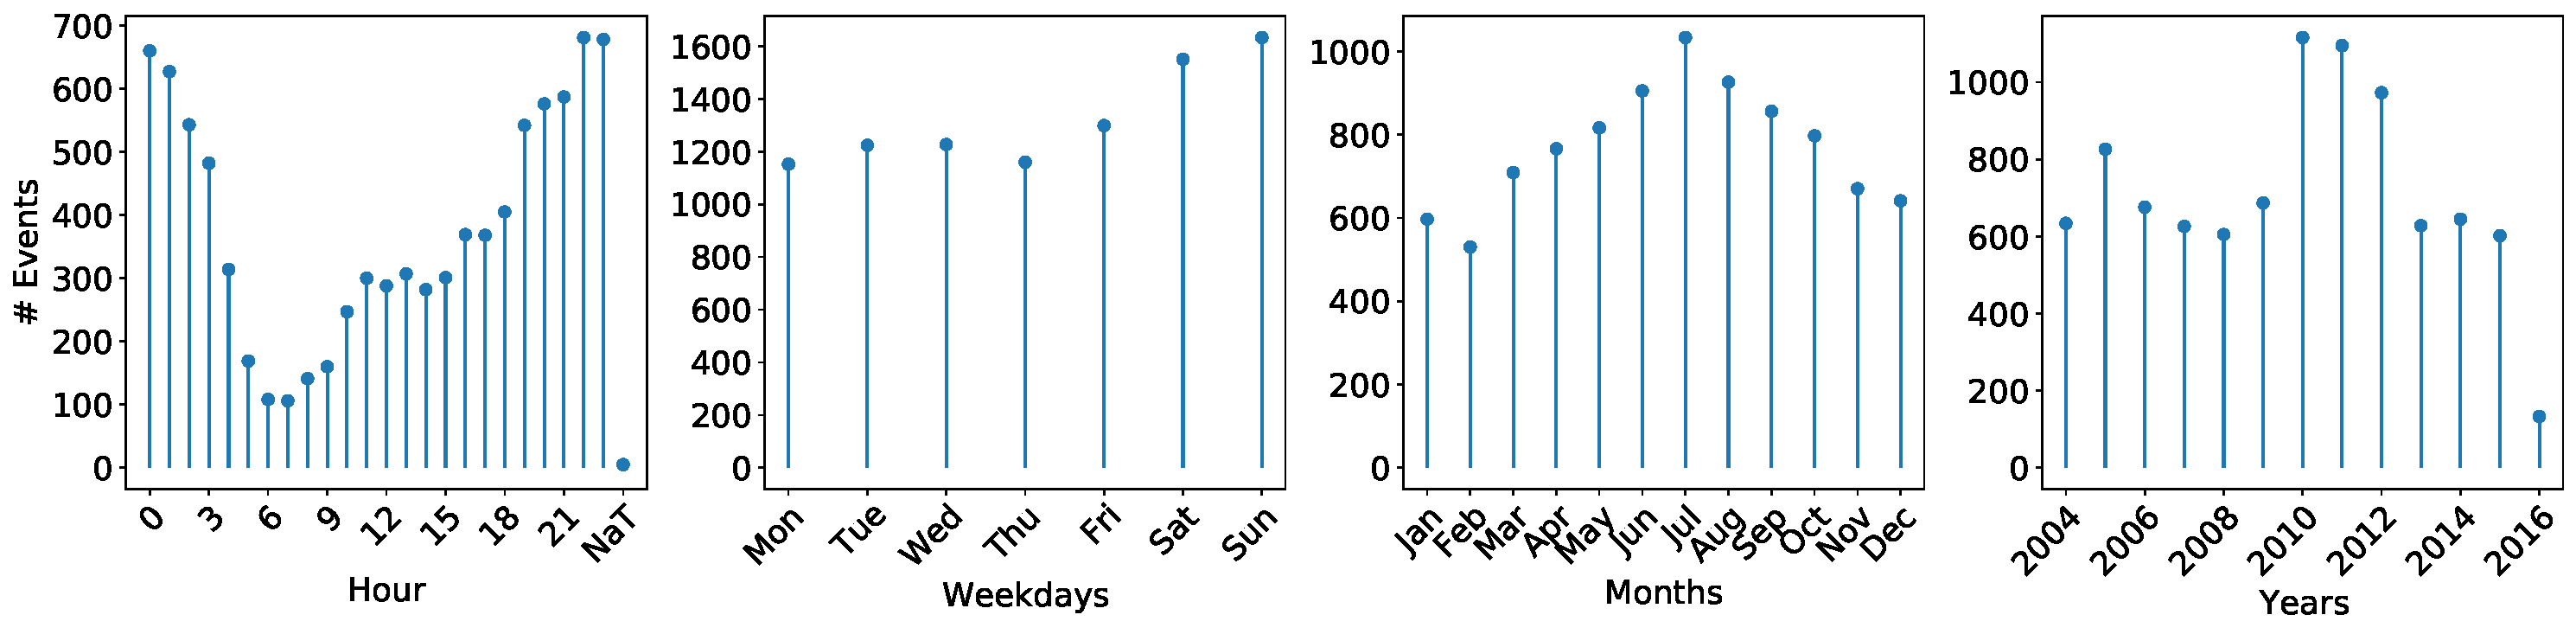
\includegraphics[width=\textwidth]{figs/trrs_times} 
	\caption{TRRs filed versus time at various scales (hour, weekday, month, year).} \label{fig:trrs_times}
\end{figure}
\begin{figure}[t!]
	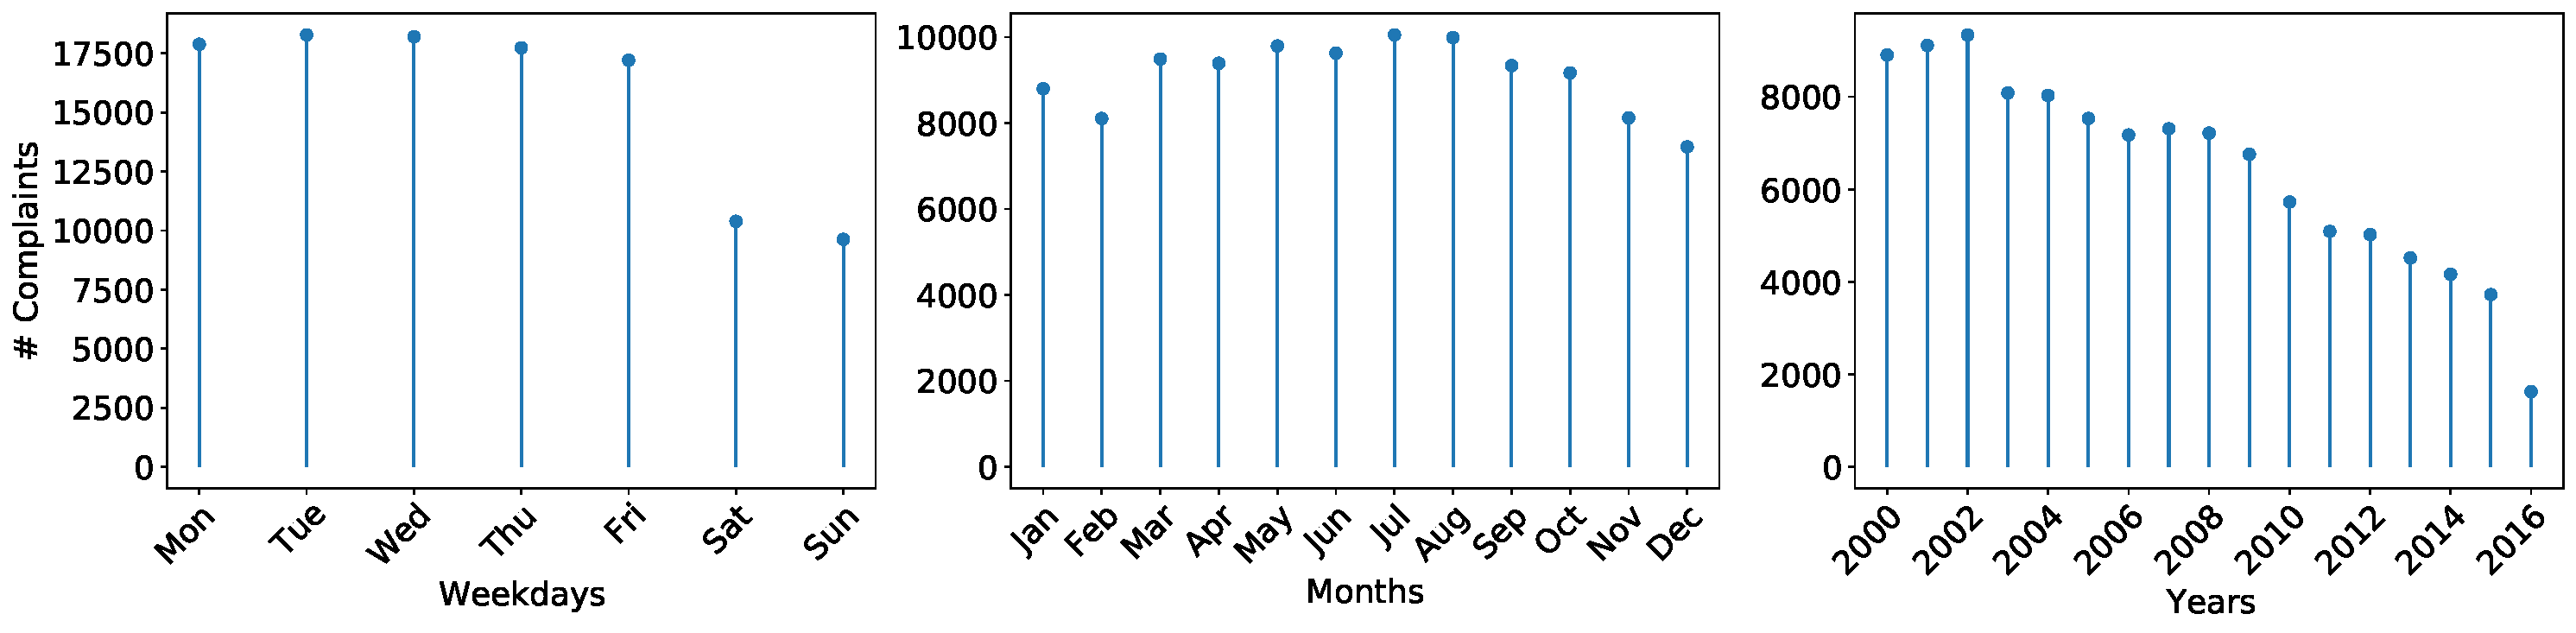
\includegraphics[width=\textwidth, clip, trim= 0 0 460 0]{figs/complaints_times} 
\caption{Complaints versus time at various scales (weekday, month)}\label{fig:complaints_times}
\end{figure}

\begin{figure}[t!] 
\begin{subfigure}{0.45\textwidth}
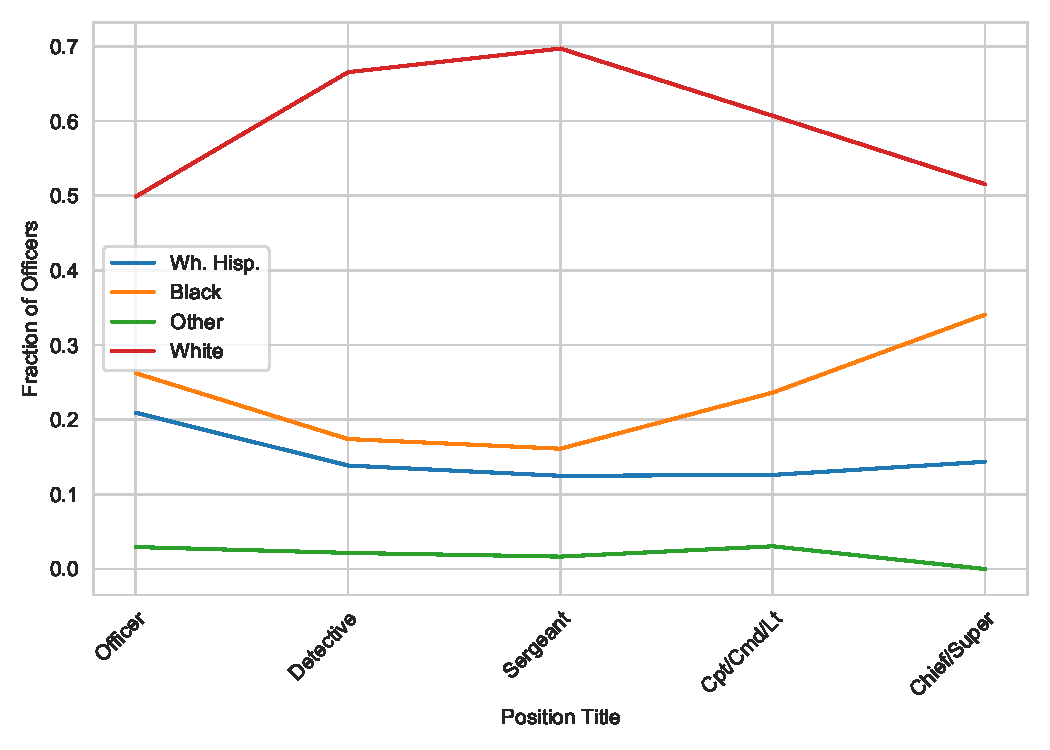
\includegraphics[width=\textwidth]{figs/position_race} 
\end{subfigure}
\begin{subfigure}{0.45\textwidth}
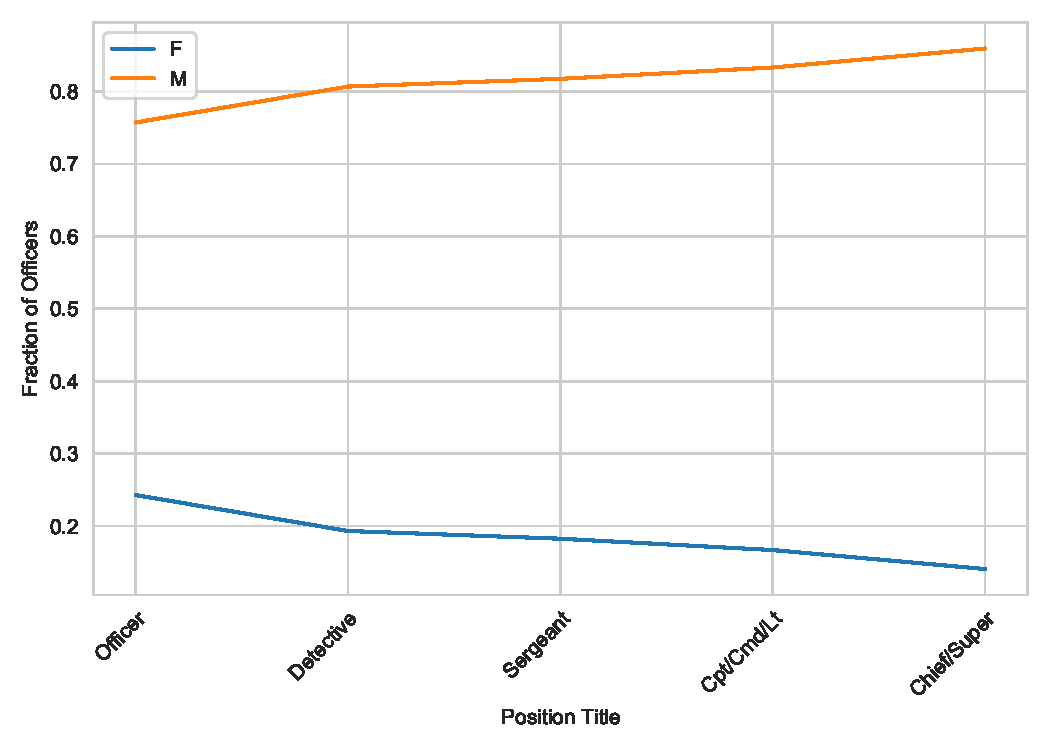
\includegraphics[width=\textwidth]{figs/position_gender} 
\end{subfigure}
\caption{Fraction of officers in representative pools of rank (Officer, Detective, Sergeant, Captain/Commander/Lieutenant, and (First) (Deputy) Chief/Superintendent)
 by race (left) and gender (right).} \label{fig:position}
\end{figure}

\begin{figure}[t!] 
	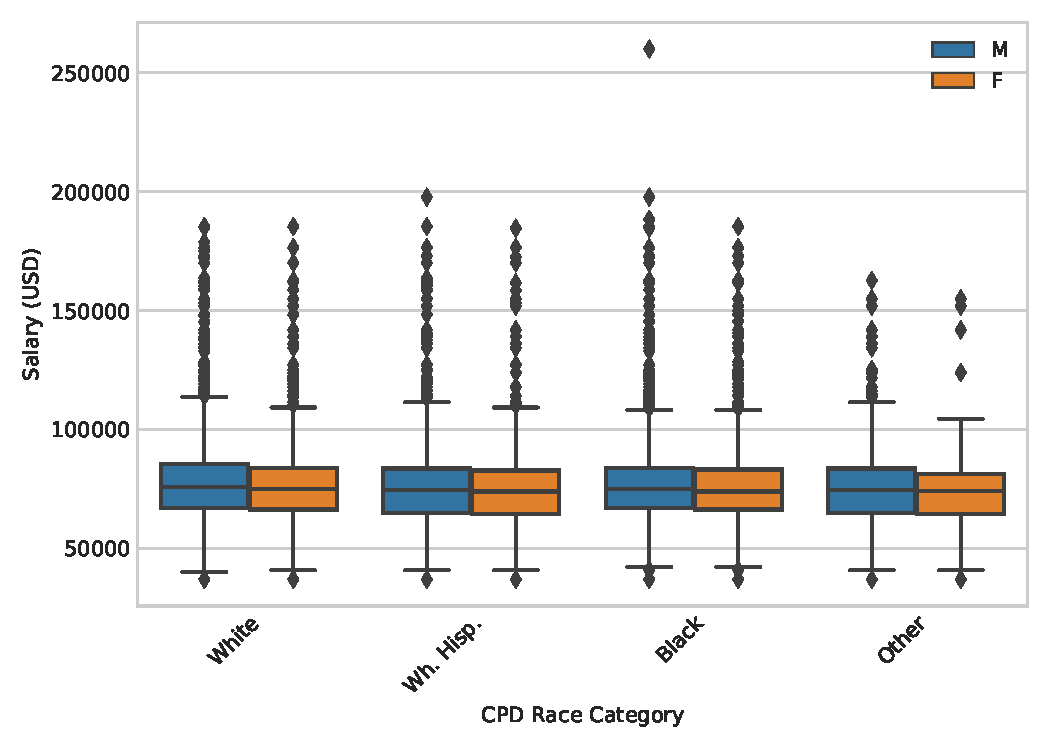
\includegraphics[width=\textwidth]{figs/salary_by_race_gender} 
	\caption{Salary (box indicates quartiles, whiskers indicate 5th/95th percentile, and scatter points are outliers) by race and gender.} \label{fig:salary_gender_race}
\end{figure}





